% Created by tikzDevice version 0.12.3.1 on 2022-09-19 12:44:23
% !TEX encoding = UTF-8 Unicode
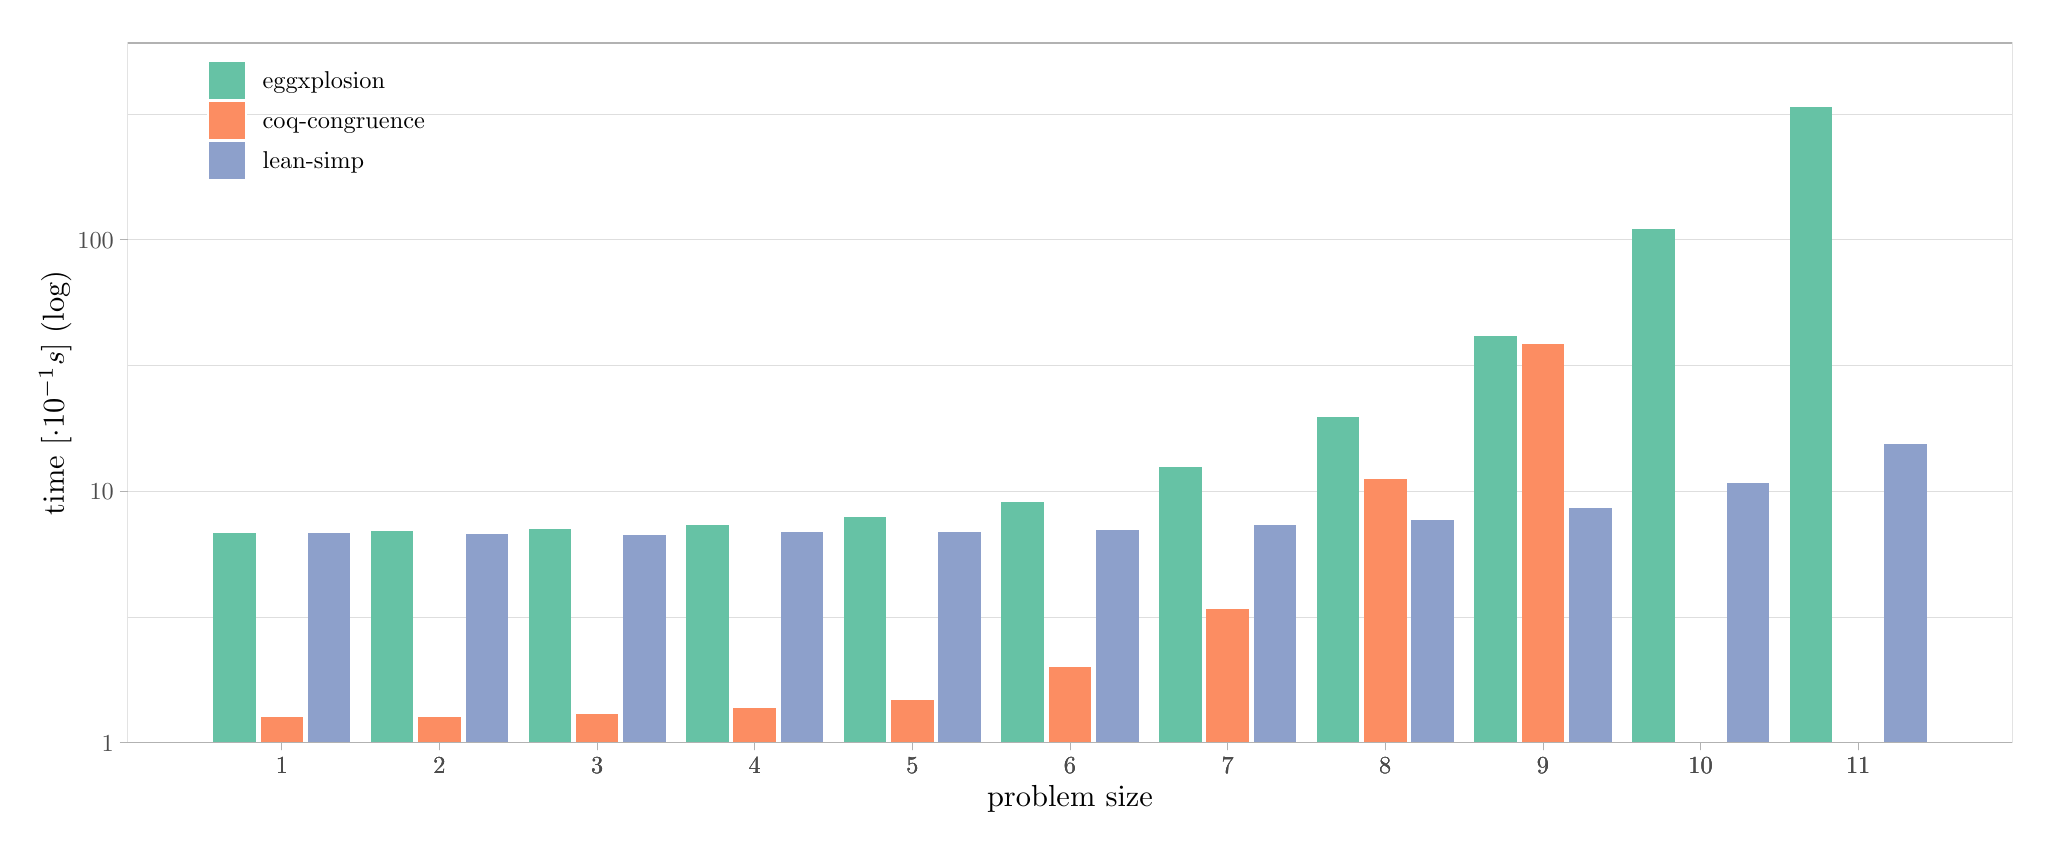
\begin{tikzpicture}[x=1pt,y=1pt]
\definecolor{fillColor}{RGB}{255,255,255}
\path[use as bounding box,fill=fillColor,fill opacity=0.00] (0,0) rectangle (722.70,289.08);
\begin{scope}
\path[clip] (  0.00,  0.00) rectangle (722.70,289.08);
\definecolor{drawColor}{RGB}{255,255,255}
\definecolor{fillColor}{RGB}{255,255,255}

\path[draw=drawColor,line width= 0.6pt,line join=round,line cap=round,fill=fillColor] (  0.00,  0.00) rectangle (722.70,289.08);
\end{scope}
\begin{scope}
\path[clip] ( 36.11, 30.69) rectangle (717.20,283.58);
\definecolor{fillColor}{RGB}{255,255,255}

\path[fill=fillColor] ( 36.11, 30.69) rectangle (717.20,283.58);
\definecolor{drawColor}{gray}{0.87}

\path[draw=drawColor,line width= 0.1pt,line join=round] ( 36.11, 76.13) --
	(717.20, 76.13);

\path[draw=drawColor,line width= 0.1pt,line join=round] ( 36.11,167.01) --
	(717.20,167.01);

\path[draw=drawColor,line width= 0.1pt,line join=round] ( 36.11,257.90) --
	(717.20,257.90);

\path[draw=drawColor,line width= 0.3pt,line join=round] ( 36.11, 30.69) --
	(717.20, 30.69);

\path[draw=drawColor,line width= 0.3pt,line join=round] ( 36.11,121.57) --
	(717.20,121.57);

\path[draw=drawColor,line width= 0.3pt,line join=round] ( 36.11,212.46) --
	(717.20,212.46);
\definecolor{fillColor}{RGB}{102,194,165}

\path[fill=fillColor] ( 67.07, 30.69) rectangle ( 82.45,106.33);
\definecolor{fillColor}{RGB}{252,141,98}

\path[fill=fillColor] ( 84.16, 30.69) rectangle ( 99.54, 40.11);
\definecolor{fillColor}{RGB}{141,160,203}

\path[fill=fillColor] (101.25, 30.69) rectangle (116.63,106.33);
\definecolor{fillColor}{RGB}{102,194,165}

\path[fill=fillColor] (124.03, 30.69) rectangle (139.41,107.17);
\definecolor{fillColor}{RGB}{252,141,98}

\path[fill=fillColor] (141.12, 30.69) rectangle (156.50, 40.12);
\definecolor{fillColor}{RGB}{141,160,203}

\path[fill=fillColor] (158.21, 30.69) rectangle (173.59,106.28);
\definecolor{fillColor}{RGB}{102,194,165}

\path[fill=fillColor] (180.99, 30.69) rectangle (196.37,108.03);
\definecolor{fillColor}{RGB}{252,141,98}

\path[fill=fillColor] (198.08, 30.69) rectangle (213.46, 41.12);
\definecolor{fillColor}{RGB}{141,160,203}

\path[fill=fillColor] (215.17, 30.69) rectangle (230.55,105.88);
\definecolor{fillColor}{RGB}{102,194,165}

\path[fill=fillColor] (237.95, 30.69) rectangle (253.33,109.48);
\definecolor{fillColor}{RGB}{252,141,98}

\path[fill=fillColor] (255.04, 30.69) rectangle (270.42, 43.10);
\definecolor{fillColor}{RGB}{141,160,203}

\path[fill=fillColor] (272.13, 30.69) rectangle (287.51,106.98);
\definecolor{fillColor}{RGB}{102,194,165}

\path[fill=fillColor] (294.92, 30.69) rectangle (310.30,112.24);
\definecolor{fillColor}{RGB}{252,141,98}

\path[fill=fillColor] (312.00, 30.69) rectangle (327.38, 46.08);
\definecolor{fillColor}{RGB}{141,160,203}

\path[fill=fillColor] (329.09, 30.69) rectangle (344.47,106.84);
\definecolor{fillColor}{RGB}{102,194,165}

\path[fill=fillColor] (351.88, 30.69) rectangle (367.26,117.75);
\definecolor{fillColor}{RGB}{252,141,98}

\path[fill=fillColor] (368.97, 30.69) rectangle (384.35, 57.99);
\definecolor{fillColor}{RGB}{141,160,203}

\path[fill=fillColor] (386.05, 30.69) rectangle (401.43,107.68);
\definecolor{fillColor}{RGB}{102,194,165}

\path[fill=fillColor] (408.84, 30.69) rectangle (424.22,130.46);
\definecolor{fillColor}{RGB}{252,141,98}

\path[fill=fillColor] (425.93, 30.69) rectangle (441.31, 79.10);
\definecolor{fillColor}{RGB}{141,160,203}

\path[fill=fillColor] (443.02, 30.69) rectangle (458.40,109.22);
\definecolor{fillColor}{RGB}{102,194,165}

\path[fill=fillColor] (465.80, 30.69) rectangle (481.18,148.50);
\definecolor{fillColor}{RGB}{252,141,98}

\path[fill=fillColor] (482.89, 30.69) rectangle (498.27,126.00);
\definecolor{fillColor}{RGB}{141,160,203}

\path[fill=fillColor] (499.98, 30.69) rectangle (515.36,111.14);
\definecolor{fillColor}{RGB}{102,194,165}

\path[fill=fillColor] (522.76, 30.69) rectangle (538.14,177.52);
\definecolor{fillColor}{RGB}{252,141,98}

\path[fill=fillColor] (539.85, 30.69) rectangle (555.23,174.72);
\definecolor{fillColor}{RGB}{141,160,203}

\path[fill=fillColor] (556.94, 30.69) rectangle (572.32,115.68);
\definecolor{fillColor}{RGB}{102,194,165}

\path[fill=fillColor] (579.72, 30.69) rectangle (595.10,216.43);
\definecolor{fillColor}{RGB}{141,160,203}

\path[fill=fillColor] (613.90, 30.69) rectangle (629.28,124.58);
\definecolor{fillColor}{RGB}{102,194,165}

\path[fill=fillColor] (636.68, 30.69) rectangle (652.06,260.59);
\definecolor{fillColor}{RGB}{141,160,203}

\path[fill=fillColor] (670.86, 30.69) rectangle (686.24,138.53);
\definecolor{drawColor}{gray}{0.70}

\path[draw=drawColor,line width= 0.6pt,line join=round,line cap=round] ( 36.11, 30.69) rectangle (717.20,283.58);
\end{scope}
\begin{scope}
\path[clip] (  0.00,  0.00) rectangle (722.70,289.08);
\definecolor{drawColor}{gray}{0.30}

\node[text=drawColor,anchor=base east,inner sep=0pt, outer sep=0pt, scale=  0.88] at ( 31.16, 27.66) {1};

\node[text=drawColor,anchor=base east,inner sep=0pt, outer sep=0pt, scale=  0.88] at ( 31.16,118.54) {10};

\node[text=drawColor,anchor=base east,inner sep=0pt, outer sep=0pt, scale=  0.88] at ( 31.16,209.42) {100};
\end{scope}
\begin{scope}
\path[clip] (  0.00,  0.00) rectangle (722.70,289.08);
\definecolor{drawColor}{gray}{0.70}

\path[draw=drawColor,line width= 0.3pt,line join=round] ( 33.36, 30.69) --
	( 36.11, 30.69);

\path[draw=drawColor,line width= 0.3pt,line join=round] ( 33.36,121.57) --
	( 36.11,121.57);

\path[draw=drawColor,line width= 0.3pt,line join=round] ( 33.36,212.46) --
	( 36.11,212.46);
\end{scope}
\begin{scope}
\path[clip] (  0.00,  0.00) rectangle (722.70,289.08);
\definecolor{drawColor}{gray}{0.70}

\path[draw=drawColor,line width= 0.3pt,line join=round] ( 91.85, 27.94) --
	( 91.85, 30.69);

\path[draw=drawColor,line width= 0.3pt,line join=round] ( 91.85, 27.94) --
	( 91.85, 30.69);

\path[draw=drawColor,line width= 0.3pt,line join=round] ( 91.85, 27.94) --
	( 91.85, 30.69);

\path[draw=drawColor,line width= 0.3pt,line join=round] (148.81, 27.94) --
	(148.81, 30.69);

\path[draw=drawColor,line width= 0.3pt,line join=round] (148.81, 27.94) --
	(148.81, 30.69);

\path[draw=drawColor,line width= 0.3pt,line join=round] (148.81, 27.94) --
	(148.81, 30.69);

\path[draw=drawColor,line width= 0.3pt,line join=round] (205.77, 27.94) --
	(205.77, 30.69);

\path[draw=drawColor,line width= 0.3pt,line join=round] (205.77, 27.94) --
	(205.77, 30.69);

\path[draw=drawColor,line width= 0.3pt,line join=round] (205.77, 27.94) --
	(205.77, 30.69);

\path[draw=drawColor,line width= 0.3pt,line join=round] (262.73, 27.94) --
	(262.73, 30.69);

\path[draw=drawColor,line width= 0.3pt,line join=round] (262.73, 27.94) --
	(262.73, 30.69);

\path[draw=drawColor,line width= 0.3pt,line join=round] (262.73, 27.94) --
	(262.73, 30.69);

\path[draw=drawColor,line width= 0.3pt,line join=round] (319.69, 27.94) --
	(319.69, 30.69);

\path[draw=drawColor,line width= 0.3pt,line join=round] (319.69, 27.94) --
	(319.69, 30.69);

\path[draw=drawColor,line width= 0.3pt,line join=round] (319.69, 27.94) --
	(319.69, 30.69);

\path[draw=drawColor,line width= 0.3pt,line join=round] (376.66, 27.94) --
	(376.66, 30.69);

\path[draw=drawColor,line width= 0.3pt,line join=round] (376.66, 27.94) --
	(376.66, 30.69);

\path[draw=drawColor,line width= 0.3pt,line join=round] (376.66, 27.94) --
	(376.66, 30.69);

\path[draw=drawColor,line width= 0.3pt,line join=round] (433.62, 27.94) --
	(433.62, 30.69);

\path[draw=drawColor,line width= 0.3pt,line join=round] (433.62, 27.94) --
	(433.62, 30.69);

\path[draw=drawColor,line width= 0.3pt,line join=round] (433.62, 27.94) --
	(433.62, 30.69);

\path[draw=drawColor,line width= 0.3pt,line join=round] (490.58, 27.94) --
	(490.58, 30.69);

\path[draw=drawColor,line width= 0.3pt,line join=round] (490.58, 27.94) --
	(490.58, 30.69);

\path[draw=drawColor,line width= 0.3pt,line join=round] (490.58, 27.94) --
	(490.58, 30.69);

\path[draw=drawColor,line width= 0.3pt,line join=round] (547.54, 27.94) --
	(547.54, 30.69);

\path[draw=drawColor,line width= 0.3pt,line join=round] (547.54, 27.94) --
	(547.54, 30.69);

\path[draw=drawColor,line width= 0.3pt,line join=round] (547.54, 27.94) --
	(547.54, 30.69);

\path[draw=drawColor,line width= 0.3pt,line join=round] (604.50, 27.94) --
	(604.50, 30.69);

\path[draw=drawColor,line width= 0.3pt,line join=round] (604.50, 27.94) --
	(604.50, 30.69);

\path[draw=drawColor,line width= 0.3pt,line join=round] (604.50, 27.94) --
	(604.50, 30.69);

\path[draw=drawColor,line width= 0.3pt,line join=round] (661.46, 27.94) --
	(661.46, 30.69);

\path[draw=drawColor,line width= 0.3pt,line join=round] (661.46, 27.94) --
	(661.46, 30.69);

\path[draw=drawColor,line width= 0.3pt,line join=round] (661.46, 27.94) --
	(661.46, 30.69);
\end{scope}
\begin{scope}
\path[clip] (  0.00,  0.00) rectangle (722.70,289.08);
\definecolor{drawColor}{gray}{0.30}

\node[text=drawColor,anchor=base,inner sep=0pt, outer sep=0pt, scale=  0.88] at ( 91.85, 19.68) {1};

\node[text=drawColor,anchor=base,inner sep=0pt, outer sep=0pt, scale=  0.88] at ( 91.85, 19.68) {1};

\node[text=drawColor,anchor=base,inner sep=0pt, outer sep=0pt, scale=  0.88] at ( 91.85, 19.68) {1};

\node[text=drawColor,anchor=base,inner sep=0pt, outer sep=0pt, scale=  0.88] at (148.81, 19.68) {2};

\node[text=drawColor,anchor=base,inner sep=0pt, outer sep=0pt, scale=  0.88] at (148.81, 19.68) {2};

\node[text=drawColor,anchor=base,inner sep=0pt, outer sep=0pt, scale=  0.88] at (148.81, 19.68) {2};

\node[text=drawColor,anchor=base,inner sep=0pt, outer sep=0pt, scale=  0.88] at (205.77, 19.68) {3};

\node[text=drawColor,anchor=base,inner sep=0pt, outer sep=0pt, scale=  0.88] at (205.77, 19.68) {3};

\node[text=drawColor,anchor=base,inner sep=0pt, outer sep=0pt, scale=  0.88] at (205.77, 19.68) {3};

\node[text=drawColor,anchor=base,inner sep=0pt, outer sep=0pt, scale=  0.88] at (262.73, 19.68) {4};

\node[text=drawColor,anchor=base,inner sep=0pt, outer sep=0pt, scale=  0.88] at (262.73, 19.68) {4};

\node[text=drawColor,anchor=base,inner sep=0pt, outer sep=0pt, scale=  0.88] at (262.73, 19.68) {4};

\node[text=drawColor,anchor=base,inner sep=0pt, outer sep=0pt, scale=  0.88] at (319.69, 19.68) {5};

\node[text=drawColor,anchor=base,inner sep=0pt, outer sep=0pt, scale=  0.88] at (319.69, 19.68) {5};

\node[text=drawColor,anchor=base,inner sep=0pt, outer sep=0pt, scale=  0.88] at (319.69, 19.68) {5};

\node[text=drawColor,anchor=base,inner sep=0pt, outer sep=0pt, scale=  0.88] at (376.66, 19.68) {6};

\node[text=drawColor,anchor=base,inner sep=0pt, outer sep=0pt, scale=  0.88] at (376.66, 19.68) {6};

\node[text=drawColor,anchor=base,inner sep=0pt, outer sep=0pt, scale=  0.88] at (376.66, 19.68) {6};

\node[text=drawColor,anchor=base,inner sep=0pt, outer sep=0pt, scale=  0.88] at (433.62, 19.68) {7};

\node[text=drawColor,anchor=base,inner sep=0pt, outer sep=0pt, scale=  0.88] at (433.62, 19.68) {7};

\node[text=drawColor,anchor=base,inner sep=0pt, outer sep=0pt, scale=  0.88] at (433.62, 19.68) {7};

\node[text=drawColor,anchor=base,inner sep=0pt, outer sep=0pt, scale=  0.88] at (490.58, 19.68) {8};

\node[text=drawColor,anchor=base,inner sep=0pt, outer sep=0pt, scale=  0.88] at (490.58, 19.68) {8};

\node[text=drawColor,anchor=base,inner sep=0pt, outer sep=0pt, scale=  0.88] at (490.58, 19.68) {8};

\node[text=drawColor,anchor=base,inner sep=0pt, outer sep=0pt, scale=  0.88] at (547.54, 19.68) {9};

\node[text=drawColor,anchor=base,inner sep=0pt, outer sep=0pt, scale=  0.88] at (547.54, 19.68) {9};

\node[text=drawColor,anchor=base,inner sep=0pt, outer sep=0pt, scale=  0.88] at (547.54, 19.68) {9};

\node[text=drawColor,anchor=base,inner sep=0pt, outer sep=0pt, scale=  0.88] at (604.50, 19.68) {10};

\node[text=drawColor,anchor=base,inner sep=0pt, outer sep=0pt, scale=  0.88] at (604.50, 19.68) {10};

\node[text=drawColor,anchor=base,inner sep=0pt, outer sep=0pt, scale=  0.88] at (604.50, 19.68) {10};

\node[text=drawColor,anchor=base,inner sep=0pt, outer sep=0pt, scale=  0.88] at (661.46, 19.68) {11};

\node[text=drawColor,anchor=base,inner sep=0pt, outer sep=0pt, scale=  0.88] at (661.46, 19.68) {11};

\node[text=drawColor,anchor=base,inner sep=0pt, outer sep=0pt, scale=  0.88] at (661.46, 19.68) {11};
\end{scope}
\begin{scope}
\path[clip] (  0.00,  0.00) rectangle (722.70,289.08);
\definecolor{drawColor}{RGB}{0,0,0}

\node[text=drawColor,anchor=base,inner sep=0pt, outer sep=0pt, scale=  1.10] at (376.66,  7.64) {problem size};
\end{scope}
\begin{scope}
\path[clip] (  0.00,  0.00) rectangle (722.70,289.08);
\definecolor{drawColor}{RGB}{0,0,0}

\node[text=drawColor,rotate= 90.00,anchor=base,inner sep=0pt, outer sep=0pt, scale=  1.10] at ( 13.08,157.13) {time [$\cdot 10^{-1} s$] (log)};
\end{scope}
\begin{scope}
\path[clip] (  0.00,  0.00) rectangle (722.70,289.08);
\definecolor{fillColor}{RGB}{255,255,255}

\path[fill=fillColor] ( 64.90,262.77) rectangle ( 79.36,277.22);
\end{scope}
\begin{scope}
\path[clip] (  0.00,  0.00) rectangle (722.70,289.08);
\definecolor{fillColor}{RGB}{102,194,165}

\path[fill=fillColor] ( 65.62,263.48) rectangle ( 78.65,276.51);
\end{scope}
\begin{scope}
\path[clip] (  0.00,  0.00) rectangle (722.70,289.08);
\definecolor{fillColor}{RGB}{255,255,255}

\path[fill=fillColor] ( 64.90,248.31) rectangle ( 79.36,262.77);
\end{scope}
\begin{scope}
\path[clip] (  0.00,  0.00) rectangle (722.70,289.08);
\definecolor{fillColor}{RGB}{252,141,98}

\path[fill=fillColor] ( 65.62,249.02) rectangle ( 78.65,262.06);
\end{scope}
\begin{scope}
\path[clip] (  0.00,  0.00) rectangle (722.70,289.08);
\definecolor{fillColor}{RGB}{255,255,255}

\path[fill=fillColor] ( 64.90,233.86) rectangle ( 79.36,248.31);
\end{scope}
\begin{scope}
\path[clip] (  0.00,  0.00) rectangle (722.70,289.08);
\definecolor{fillColor}{RGB}{141,160,203}

\path[fill=fillColor] ( 65.62,234.57) rectangle ( 78.65,247.60);
\end{scope}
\begin{scope}
\path[clip] (  0.00,  0.00) rectangle (722.70,289.08);
\definecolor{drawColor}{RGB}{0,0,0}

\node[text=drawColor,anchor=base west,inner sep=0pt, outer sep=0pt, scale=  0.88] at ( 84.86,266.96) {eggxplosion};
\end{scope}
\begin{scope}
\path[clip] (  0.00,  0.00) rectangle (722.70,289.08);
\definecolor{drawColor}{RGB}{0,0,0}

\node[text=drawColor,anchor=base west,inner sep=0pt, outer sep=0pt, scale=  0.88] at ( 84.86,252.51) {coq-congruence};
\end{scope}
\begin{scope}
\path[clip] (  0.00,  0.00) rectangle (722.70,289.08);
\definecolor{drawColor}{RGB}{0,0,0}

\node[text=drawColor,anchor=base west,inner sep=0pt, outer sep=0pt, scale=  0.88] at ( 84.86,238.06) {lean-simp};
\end{scope}
\end{tikzpicture}
